\documentclass[11pt,a4paper]{article} 

\usepackage[dutch]{babel} %needs to specified for minutes package (else it will be in German)
\usepackage{a4wide}%For a wider spacing of the text (smaller left/right margin)
\usepackage{graphicx}
\usepackage{setspace}
\usepackage{minutes}

\pagestyle{plain}
\usepackage{todositemized}
%more memmorable commands to make the checked and crossed symbols





%%%%%%%%%%%%%%%%%%%%%%%%%%%%%%%%%%%%%%%%%%%%%%%%%%%%%%%%%%%%%%%%%%%%%%%%%%%%%%%
%
% Important: This template compiles without errors
% always check errors, also the yellow ones, even if you get a PDF
%
%%%%%%%%%%%%%%%%%%%%%%%%%%%%%%%%%%%%%%%%%%%%%%%%%%%%%%%%%%%%%%%%%%%%%%%%%%%%%%%%





\newpage



\usepackage[dutch]{babel} %needs to specified for minutes package (else it will be in German)
\usepackage{a4wide}%For a wider spacing of the text (smaller left/right margin)

\usepackage{setspace}
\usepackage{minutes}

\pagestyle{plain}
\usepackage{todositemized}
%more memmorable commands to make the checked and crossed symbols





%%%%%%%%%%%%%%%%%%%%%%%%%%%%%%%%%%%%%%%%%%%%%%%%%%%%%%%%%%%%%%%%%%%%%%%%%%%%%%%
%
% Important: This template compiles without errors
% always check errors, also the yellow ones, even if you get a PDF
%
%%%%%%%%%%%%%%%%%%%%%%%%%%%%%%%%%%%%%%%%%%%%%%%%%%%%%%%%%%%%%%%%%%%%%%%%%%%%%%%%



\begin{document}

\begin{Minutes}{Notulen Poject Natuurkunde, groepje 24}


%Add relevant date, time and location here
\minutesdate{16-06-2023} %Write the date of when you finish the minutes
\starttime{11:00}
\endtime{}
\location{}

%Add relevant names here
\participant{Tom, Noah} 
\minutetaker{Tom}

% \moderation{Niemand} 
%In case people are not present


\maketitle



\newpage


\section{Mededelingen} 
We begonnen vandaag om 11 uur. De rheometer is vandaag voor het grootste deel van de dag ingenomen, dus moeten we waarschijnlijk de metingen morgen doen. Tom heeft een begin gemaakt aan het begrijpen hoe manim precies werkt. Later op de dag hebben Noah en Tom nog eens gekeken naar een fit waar Noah mee bezig was, het bleek dat er een paar rekenfouten in zaten waardoor de waardes een onjuiste orde van grootte hadden. Dit hebben ze daarna opgelost. Daarna gingen we kijken naar het nieuwe artikel dat Noah en Antoine vorige keer hadden besproken. Daarin stond een andere formule dan de formule die eerder was gebruikt. Toen we deze formule hadden gebruikt om onze waardes in te vullen, klopte de grafiek weer. De rest van de dag heeft Noah gewerkt aan een fit en heeft Tom de template voor de poster afgemaakt. Talha is absent in verband met overleden familielid.


\section{Wat moeten we nu doen/bespreken?}
We moeten van de medium en soft putty in ieder geval de 20 graden en -30 graden metingen doen met de rheometer en voor de extra soft putty alleen de -30 graden metingen.

\section{Figure}
\begin{figure}[h]
    \centering
    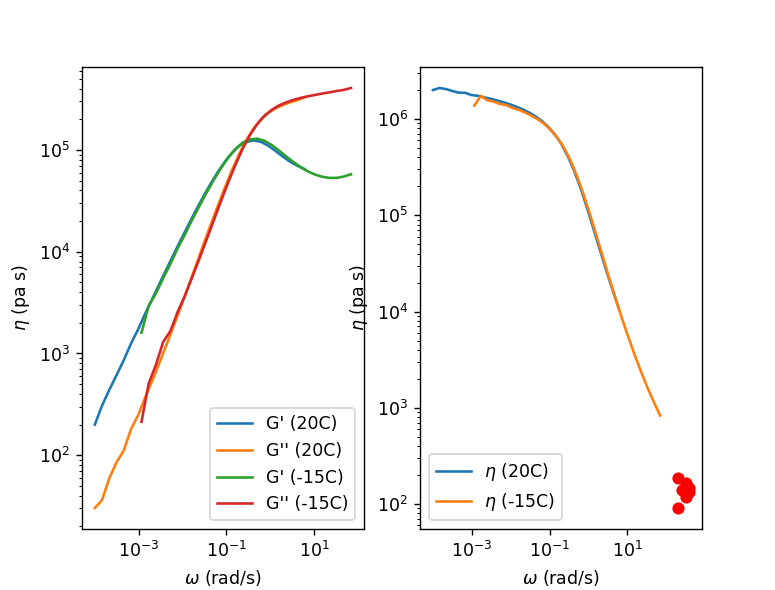
\includegraphics[width=0.5\linewidth]{Werkend.png}
    \caption{Hier is dezelfde grafiek te zien als van 12 juni alleen nu hebben we onze verkregen data (rode punten) toegevoegd van de putty. Wat te zien is dat we niet genoeg data uit de rheometer hebben gekregen om de viscositeit van onze putty te beschrijven, door nog een meting op -30 graden te doen hopen we deze te verkijgen. Wel is te zien dat als de trend van de rheometer data wordt voortgezet de lijn ongeveer met onze data zal overlappen.}
    \label{fig:enter-label}
\end{figure}

\end{Minutes}
\end{document}




\section{Oude actiepunten}
Zijn er niet.

\section{Wat moeten we nu doen/bespreken?}

\subsection{Wie wil en kan wat?}

\task{talha}{checklist}

\subsection{Communicatie}


\subsection{Beschikbaarheid}


\section{Checklist uit de Powerpoint}



\section{Overige punten}
We wachten even morgen af, als we met Antoine spreken.

\section{Nieuwe actiepunten}
\listoftasks
\section{Volgende vergadering}
De volgende bijeenkomst is morgen met de begeleider, bij het fancy koffiezet apparaat bij D.

\section{Afsluiting vergadering}
De vergadering is om 12:49 gesloten.


\end{Minutes}
\end{document}